\documentclass[a4paper]{article}

\usepackage[english]{babel}
\usepackage[utf8x]{inputenc}
\usepackage[framemethod=pstricks]{mdframed}
\usepackage{showexpl}
\usepackage[xindy]{glossaries}
\usepackage{float}

\newcommand{\bgls}[1]{\textbf{\gls{#1}}}
\newcommand{\bglspl}[1]{\textbf{\glspl{#1}}}

\makeglossaries
\newglossaryentry{update transaction}
{
name={Update Transaction},
description={A message signed by both parties that updates the state of a channel. This is posted to the bank or blockchain to close the channel, however an infinite number of them can be exchanged between the two parties before then}
}

\newglossaryentry{opening transaction}
{
name={Opening Transaction},
description={A message signed by both parties that creates a channel. This is posted to the bank or blockchain and serves to identify the parties and place funds in escrow}
}

\newglossaryentry{net transfer amount}
{
name={Net Transfer Amount},
description={An amount included in \bglspl{update transaction} which specifies how much money to transfer from \textbf{Party 1} to \textbf{Party 2} when the channel closes. If it is negative, funds are transferred in the other direction}
}

\newglossaryentry{conditional transfer amount}
{
name={Conditional Transfer Amount},
description={An amount included in \bglspl{smart condition}, which is added to the channel's \bgls{net transfer amount} if a \bgls{fulfillment} is posted which causes the \bgls{smart condition} to return true}
}

\newglossaryentry{nonce}
{
name={Nonce},
description={An integer included the \bgls{update transaction} which is incremented with each new \bgls{update transaction}. This is used by the bank or the blockchain to ascertain the ordering of \bglspl{update transaction}. An \bgls{update transaction} with a higher \bgls{nonce} will always override one with a lower \bgls{nonce}}
}

\newglossaryentry{hold period}
{
name={Hold Period},
description={A time period included the \bgls{update transaction}. The bank or blockchain must wait this amount of time before transferring any money when the channel is closed. This provides a chance for one of the parties to counteract a cheating attempt where the other party posts an old \bgls{update transaction}. If a newer \bgls{update transaction} with a higher \bgls{nonce} is posted before the \bgls{hold period} is over, it will override the older one}
}

\newglossaryentry{smart condition}
{
name={Smart Condition},
description={A piece of Turing-complete code included in the \bgls{update transaction} that is evaluated by the bank or blockchain during the \bgls{hold period}. It can return either true or false when supplied with a \bgls{fulfillment}. It has an associated \bgls{conditional transfer amount}, which is added to the channel's \bgls{net transfer amount} if the \bgls{smart condition} returns true}
}

\newglossaryentry{fulfillment}
{
name={Fulfillment},
description={A piece of data to be evaluated by a \bgls{smart condition}. This can be posted at any time during the \bgls{hold period}, and only needs to be signed by one of the parties}
}

\newglossaryentry{payment secret}
{
name={Payment Secret},
description={A secret shared between the source and destination of a multihop payment. It is hashed and used to create \bglspl{hashlock condition} between all the intermediary nodes involved in the multihop payment. The destination reveals it to the last intermediary node to claim the payment, and the last intermediary nodes reveals it to the second-to-last and so on back to the source}
}

\newglossaryentry{hashlock condition}
{
name={Hashlock Condition},
description={A \bgls{smart condition} that hashes its argument, usually a \bgls{payment secret} and compares the hash to a prespecified string. If it matches, the \bgls{smart condition} returns true and adds its \bgls{conditional transfer amount} to the channel's \bgls{net transfer amount}}
}

\newglossaryentry{payment initialization}
{
name={Payment Initialization},
description={A message sent from the source of a multihop payment to the destination, setting up the payment and conveying the \bgls{payment secret} and the \textbf{Amount} of the payment}
}

\newglossaryentry{routing message}
{
name={Routing Message},
description={A message propagated between nodes as part of the routing protocol. It contains the hash of the \bgls{payment secret} and an \textbf{Amount}, which is added to by each node that propagates it}
}

\newglossaryentry{routing table}
{
name={Routing Table},
description={A table maintained by each node that records \bglspl{routing message} received and forwarded by that node. It is used to route the payment corresponding to a given \bglspl{routing message}}
}

\mdfdefinestyle{message}
{
  nobreak=true,
  leftmargin=10,
  rightmargin=10,
  innerleftmargin=20,
  innerrightmargin=20,
  innertopmargin=10,
  innerbottommargin=10,
  skipabove=20pt,
  skipbelow=20pt
}

\setlength{\parskip}{3pt}

\newenvironment{mydescription}
{\begin{description}
\setlength{\itemsep}{5pt}
  \setlength{\parskip}{0pt}
  \setlength{\labelsep}{5pt}
}{
\end{description}}

\title{Universal Payment Channels}
\author{Jehan Tremback\\
\texttt{jehan.tremback@gmail.com}\\}
\date{November 2015\\
\texttt{v0.4}}

\begin{document}
\maketitle

\begin{abstract}
Payment channels are a type of private ledger, backed by assets held by a bank, payment processor, or blockchain. We use payment channels to specify a payment network which allows for instant transfers of conventional currencies, cryptocurrencies, and any other kind of asset which can be owned without physical possession. The network can, in many circumstances, convert one asset type into another without using exchanges. For example, Dollars to Dogecoins, or Bitcoins to grain futures. Payments are made directly between nodes in the network, without involving the entities or blockchains backing it. This greatly reduces load on these entities and blockchains, allowing for massive scalability.

The heart of this network is the Reactive Payment Routing (RPR) protocol, based on the packet routing protocols that power the internet. RPR allows the network to automatically find the cheapest route for any payment. Because of this, RPR is also able to find the best exchange rate between any two asset types used on the network.

UPC's payment channels also can process Turing-complete "smart conditions", making the network extensible and allowing developers to create a new class of payment channel applications.
\end{abstract}

\section*{Introduction}

This paper concerns a payment network called Universal Payment Channels, or UPC. UPC can handle transfers of any type of conventional or crypto currency, as well as physical or virtual goods, as long as these goods can be considered owned without physical possesion and kept in escrow. Furthermore, UPC routes payments across stores of value, with the network automatically arriving at the market exchange rate.

The vast majority of UPC payments are made without interfacing with any third party ledger, such as a bank or blockchain. This means that there can be an almost unlimited amount of payments that do not put any strain on bank servers, or add anything to the blockchain. The only time that the bank or the blockchain is involved is when a network participant wants to take money out of the network, or put money into it.

This makes it very easy for application developers to interface with UPC. Instead of interfacing with a bank or payment processor, the only thing that an application needs to do is to send cryptographically signed messages on behalf of the user. For example, there is software in development using UPC to allow internet backbone routers to pay one another per-packet, many times each second. These payments can be sent or received in dollars, Dogecoins, or any other currency. Even though the volume of payments created by this type of software is oceanic, the banks and blockchains backing up the network are rarely contacted.

UPC consists of a series of ``channels'' between network participants. A channel is a private ledger arrangement between any two parties and a blockchain, a bank, or some other kind of institution. It allows the parties to exchange payment trustlessly, by sending updated ledger balances to one another (not to the bank or blockchain). At any time, each of the participants can be confident that they will be able to retrieve every cent or Satoshi that they are owed.

UPC's key innovation is Reactive Payment Routing (RPR), a routing protocol inspired by the protocols that power the internet. UPC uses RPR to route payments across interconnected channels, finding the cheapest path.

The Internet is a \emph{packet-switched network}. Any computer on the Internet can reach any other computer, and the network grows organically and routes around damage. Routing protocols ensure that each packet takes the fastest path through the network.

UPC is a \emph{payment-switched network}. Any network participant can pay any other, and UPC grows organically and routes around damage. UPC ensures that each payment takes the cheapest path through the network.

\section*{Related work}
Payment channels are, at root, based on the idea of commercial credit. One of the main purposes of commercial credit is to allow two parties to consolidate a large number of smaller payments into one larger payment which is made periodically. Clearinghouses extend this instrument by placing funds in escrow so that two parties can exchange a large number of transactions without having to trust each other.

Some of the first formalization of the role of a clearinghouse into the concept of a payment channel occurred in the Bitcoin community with Mike Hearn's work on micropayment channels\cite{btcwiki}\cite{bitcoinj}, Alex Aakselrod's work on chained micropayment channels\cite{blueadept} and C. J. Plooy's system Amiko Pay\cite{amiko}. Further innovation appeared with Poon and Dryja's Lightning Network\cite{lightning} and Decker and Wattenhofer's Duplex Channels\cite{duplexchannels}. All of these protocols are designed for Bitcoin, whose limited scripting capabilities demand complicated specifications. Interledger\cite{interledger} is the only protocol we know of specifying a multihop payment channel system generalized across stores of value. It is a bit more complex than the protocol in this paper, but includes a formal specification. Zackary Hess's work in Flying Fox\cite{flyingfox} deserves special mention, because his channel specification forms the basis of the one in this paper.

None of the above work includes the two key innovations in this paper: Turing-complete \bglspl{smart condition} (``smart contracts'' are a similar concept), and the Reactive Payment Routing (RPR) protocol, which is necessary for an actual working payment network. RPR is partially based on Ad hoc On-Demand Distance Vector Routing (AODV)\cite{aodv}, however it is simpler and provides full network anonymity for all nodes participating in a payment route.

\section{Basic channel}

A channel is created when two parties create and sign an \bgls{opening transaction} to put money from both parties in escrow with an institution such as a bank, or lock up coins on a blockchain. The money is put into escrow with the understanding that at some point in the future it will be transferred back to the parties upon receipt of an \bgls{update transaction} signed by both parties. This \bgls{update transaction} has a special number on it called a ``nonce'', and specifies two additional actions to take before transferring the funds back to the parties:

\begin{enumerate}
\item Adjust the amounts that both parties have in escrow, lowering one amount and raising the other by the same amount. This effectively transfers funds from one party to the other.
\item Wait for a certain \bgls{hold period} before releasing the funds to back to the parties. If someone gives you another \bgls{update transaction} signed by both parties, and this transaction's nonce is higher, throw the current \bgls{update transaction} out and use the new one, restarting the \bgls{hold period}.
\end{enumerate}

Alice and Bob exchange \bglspl{update transaction} back and forth, changing the amount of funds to be transferred to make payments to one another. Each time they make a new \bgls{update transaction}, they increment the nonce. To accept a payment, both of them sign it.

\begin{itemize}
\item If Bob disappears, Alice can post the last signed \bgls{update transaction} and collect the money owed her without Bob's involvement, after the hold period is over.

\item If Bob tries to cheat by posting an old \bgls{update transaction} where he's doing better than he is currently, Alice can post the latest \bgls{update transaction}, which will override the old one. As long as Alice checks whether Bob has posted an old \bgls{update transaction} at least once every \bgls{hold period}, she can post the latest \bgls{update transaction} and stop him from cheating.
\end{itemize}


\subsection{Opening Transaction}

A channel is opened with an \bgls{opening transaction}. The \bgls{opening transaction} serves to identify the channel and the parties, and place the money in escrow. This could be sent to a bank, or supplied to a smart contract on a blockchain.

\begin{mdframed}[style=message]
\begin{mydescription}
\item[Opening Transaction:] \hfill
  \begin{mydescription}
  \item[Party 1:] Public key or other signature verification information for one of the participants.
  \item[Party 2:] Public key or other signature verification information for the other participant.
  \item[Amount 1:] The amount of money that \textbf{Party 1} has placed in the channel
  \item[Amount 2:] The amount of money that \textbf{Party 2} has placed in the channel
  \end{mydescription}
\item[Signature 1:] \textbf{Party 1}'s signature on \bgls{opening transaction}
\item[Signature 2:] \textbf{Party 2}'s signature on \bgls{opening transaction}
\end{mydescription}
\end{mdframed}

\subsection{Update Transaction}

\bglspl{update transaction} are sent back and forth between \textbf{Party 1} and \textbf{Party 2} and serves to transfer the money. Only the last of these \bglspl{update transaction} should be posted to the bank or blockchain. When an \bgls{update transaction} is posted, it always results in the closure of the channel (whether it is honored, or a higher-nonced \bgls{update transaction} is honored).

\begin{mdframed}[style=message]
\begin{mydescription}
  \item[Update Transaction:] \hfill
    \begin{mydescription}
      \item[Nonce:] A number which is incremented with each new \bgls{update transaction}.
      \item[Net Transfer Amount:] The amount of money to transfer from \textbf{Party 1} to \textbf{Party 2} (can be negative).
      \item[Hold Period:] An amount of time (or number of blocks) to wait before closing the channel and transferring funds, after a \bgls{update transaction} has been published
    \end{mydescription}
  \item[Signature 1:] \textbf{Party 1}'s signature on \bgls{update transaction}
  \item[Signature 2:] \textbf{Party 2}'s signature on \bgls{update transaction}
\end{mydescription}
\end{mdframed}

\subsubsection{Making payments}

To make payments to one another, Alice and Bob pass signed \bglspl{update transaction} back and forth.

If Alice wants to pay Bob, she adjusts the \bgls{net transfer amount}, signs the \bgls{update transaction}, then passes it to Bob. None of this involves the \bgls{update transaction} being shown to anyone else, and can happen instantly. Alice and Bob can do this as many times as they want.

To actually claim the funds, either party posts the latest \bgls{update transaction}. After \bgls{hold period} is over, the channel closes: the \bgls{net transfer amount} is subtracted from \textbf{Amount 1} and added to \textbf{Amount 2}, and the amounts are transferred back to the accounts of the participants.

This means that if Alice disappears or becomes uncooperative, Bob can still get his money out by posting the last valid \bgls{update transaction} he has and waiting for the \bgls{hold period} to end.

\subsubsection{Stopping cheaters}

If a \bgls{update transaction} with a higher \bgls{nonce} is published before the \bgls{hold period} ends, it overrides the older \bgls{update transaction}.

If Bob tries to cheat by publishing an old \bgls{update transaction} where he has a higher amount than he does currently, Alice can simply publish the newer \bgls{update transaction}, which will have a higher \bgls{nonce}.

Another option is to punish Bob by transferring all his funds to Alice if she is able to post a higher-nonced \bgls{update transaction} after him. This makes a cheating attempt riskier and may be beneficial in some situations.

\section{Smart Conditions}

\bglspl{smart condition} are pieces of Turing-complete code that are evaluated by the bank or blockchain during the \bgls{hold period}. They can return either true or false when supplied with a piece of data, which is referred to as a \bgls{fulfillment}. They have an associated \bgls{conditional transfer amount}, which is added to the channel's \bgls{net transfer amount} if the \bgls{smart condition} returns true.

\bglspl{update transaction} can have a list of \bglspl{smart condition}. A \bgls{smart condition} consists of the \bgls{conditional transfer amount} and the \textbf{Function} which takes an argument and returns either true or false. The \textbf{Function} does not have any side effects, it is a pure function.

\begin{mdframed}[style=message]
\begin{mydescription}
\item[Update Transaction:] \hfill
  \item[Nonce:] A number which is incremented with each new \bgls{update transaction}.
  \item[Net Transfer Amount:] The amount of money to transfer from \textbf{Party 1} to \textbf{Party 2} (can be negative).
  \item[Hold Period:] An amount of time (or number of blocks) to wait before closing the channel and transferring funds, after an \bgls{update transaction} has been posted.
  \begin{mydescription}
  \item[Conditions:] \hfill
    \begin{mydescription}
    \item[1:] \hfill
      \begin{mydescription}
      \item[Conditional Transfer Amount:] Add this to the channel's \bgls{net transfer amount} if \textbf{Function} returns true.
      \item[Function(argument):] Takes an argument and returns either true or false
      \end{mydescription}
    \item[2:] \ldots
    \end{mydescription}
  \end{mydescription}
\end{mydescription}
\end{mdframed}

Pieces of data called \bglspl{fulfillment} can be posted during the \bgls{hold period}. These act to ``fulfill'' the ``conditions''. \bglspl{fulfillment} only need to be signed by one of the channel participants.

\begin{mdframed}[style=message]
\begin{mydescription}
\item[Fulfillment:] \hfill
  \begin{mydescription}
  \item[Condition:] Which condition does this fulfill?
  \item[Argument:] Data with which to evaluate the \bgls{smart condition}.
  \end{mydescription}
\end{mydescription}
\end{mdframed}

When a \bgls{fulfillment} is posted, it is evaluated by the corresponding \bgls{smart condition}. If the \bgls{smart condition} evaluates to true, the \bgls{conditional transfer amount} is added to the channel's \bgls{net transfer amount}, and the \bgls{smart condition} is removed from the list.

\subsection{Gas}
Notice that one channel participant could send the other a \bgls{smart condition} that resulted in an infinite loop or other excessive use of resources. Blockchain-based smart contract systems like Ethereum\cite{ethereum} or Tendermint\cite{tendermint} use a concept of ``gas'' where each step of code execution costs a small amount. Execution aborts if there is insufficient gas. Such a gas scheme could be specified here, but we believe that it is an implementation detail, and outside of the scope of this specification.

Whatever the gas scheme used, nodes could be required to pay gas upon posting a \bgls{fulfillment}. This way incentives are aligned so that the party who would like a certain condition evaluated pays for it.

\subsection{Using Smart Conditions}

\bglspl{smart condition} can be used to implement complex logic over channels to give them enhanced capabilities. Here is how Alice and Bob would implement a ``hashlock'' \bgls{smart condition}. Specifically, Alice wants to guarantee that she will transfer 32 coins to Bob if he can supply a string (referred to as a \bgls{payment secret}) that hashes to ``59A1904325CCB''. Alice is \textbf{Party 1} and Bob is \textbf{Party 2}.

\begin{mdframed}[style=message]{\emph{Alice to Bob}}
\begin{mydescription}
\item[Update Transaction:] \hfill
  \begin{mydescription}
    \item[Nonce:] 12
    \item[Net Transfer Amount:] -34
    \item[Hold Period:] 8
    \item[Conditions:] \hfill
      \begin{mydescription}
        \item[1:] \hfill
          \begin{mydescription}
            \item[Conditional Transfer Amount:] 32
            \item[Function(secret):] \texttt{\\ if sha3(secret) is equal to\\ "59A1904325CCB", return true;\\ else return false}
  \end{mydescription}
    \end{mydescription}
  \end{mydescription}
\item[Signature 1:] Alice's signature on \bgls{update transaction}
\end{mydescription}
\end{mdframed}

\subsubsection{Closing the channel}

If Bob wants to close the channel at this point, he posts the \bgls{update transaction}, along with his and Alice's signatures. To fulfill the \bgls{smart condition} and have the \bgls{conditional transfer amount} added to the channel's \bgls{net transfer amount}, Bob must post a \bgls{fulfillment} that causes the \bgls{smart condition} to return true during the \bgls{hold period}. Note that the \bgls{fulfillment} only needs to be signed by the party posting it.

\begin{mdframed}[style=message]{\emph{Along with the above \bgls{update transaction}, Bob posts}}
\begin{mydescription}
  \item[Fulfillment:] \hfill \begin{mydescription}
    \item[Condition:] 1
    \item[Argument:] ``theSecret''
  \end{mydescription}
  \item[Signature:] Bob's signature on \bgls{fulfillment}
\end{mydescription}
\end{mdframed}

\subsubsection{Fulfilling the condition without closing the channel}

Of course, most of the time Bob doesn't want to close the channel right away. Bob can now prove that he could unlock the money if he wanted, so Alice might as well adjust the channel's \bgls{net transfer amount} as specified by the \bgls{smart condition}. Bob sends the \bgls{payment secret} to Alice, who adjusts the channel's \bgls{net transfer amount}, increments the \bgls{nonce}, removes condition 1, and signs a new \bgls{update transaction}.

\begin{mdframed}[style=message]{\emph{Bob to Alice}}
\begin{mydescription}
\item[Fulfillment:] \hfill
\begin{mydescription}
  \item[Condition:] 1
  \item[Argument:] ``theSecret''
\end{mydescription}
\item[Signature:] Bob's signature on \bgls{fulfillment}
\end{mydescription}
\end{mdframed}

\begin{mdframed}[style=message]{\emph{Both sign}}
\begin{mydescription}
\item[Update Transaction:] \hfill
\begin{mydescription}
  \item[Nonce:] 13
  \item[Net Transfer Amount:] -2
  \item[Hold Period:] 8
\end{mydescription}
\item[Signature 1:] Alice's signature
\item[Signature 2:] Bob's signature
\end{mydescription}
\end{mdframed}

\subsubsection{Canceling the condition}

Similarly, Bob can inform Alice that he will never be able to provide the secret. In this case there is no reason for them to keep passing a condition that will never be fulfilled back and forth. Bob simply makes a new \bgls{update transaction}, without the \bgls{smart condition}.

\begin{mdframed}[style=message]{\emph{Both sign}}
\begin{mydescription}
\item[Update Transaction:] \hfill
\begin{mydescription}
  \item[Nonce:] 13
  \item[Net Transfer Amount:] -34
  \item[Hold Period:] 8
\end{mydescription}
\item[Signature 1:] Alice's signature on \bgls{update transaction}
\item[Signature 2:] Bob's signature on \bgls{update transaction}
\end{mydescription}
\end{mdframed}

\section{Multihop payments}

With the help of a hashlock condition, it is possible to trustlessly route payments across multiple hops. Let's say that Alice would like to transfer some funds to Charlie, but she does not have a channel open with him. If she has a channel with Bob, and Bob has a channel with Charlie, the funds can be transferred.

First, Alice sends a \bgls{payment secret} to Charlie:

\begin{mdframed}[style=message]{\emph{Alice to Charlie}}
\begin{mydescription}
\item[Payment Secret:] ``theSecret''
\end{mydescription}
\end{mdframed}

Then, Alice sends a hashlocked payment to Bob:

\begin{mdframed}[style=message]{\emph{Alice to Bob}}
\begin{mydescription}
\item[Update Transaction:] \hfill
\begin{mydescription}
  \item[Nonce:] 13
  \item[Net Transfer Amount:] -2
  \item[Hold Period:] 8
  \item[Conditions:] \hfill
  \begin{mydescription}
    \item[1:] \hfill
    \begin{mydescription}
      \item[Conditional Transfer Amount:] -101
      \item[Function(secret):] \texttt{\\ if sha3(secret) is equal to\\ "73B88F8C24EAA", return true;\\ else return false}
    \end{mydescription}
  \end{mydescription}
\end{mydescription}
\item[Signature 1:] Alice's signature on \bgls{update transaction}
\end{mydescription}
\end{mdframed}

Notice that Alice has sent Bob 101 coins instead of 100, as Bob charges her a 1\% fee for routing payments.

Now, Bob sends the payment along to Charlie (Bob is \textbf{Party 1} and Charlie is \textbf{Party 2} in their channel):

\begin{mdframed}[style=message]{\emph{Bob to Charlie}}
\begin{mydescription}
\item[Update Transaction:] \hfill
\begin{mydescription}
  \item[Nonce:] 42
  \item[Net Transfer Amount:] 56
  \item[Hold Period:] 10
  \item[Conditions:] \hfill
  \begin{mydescription}
    \item[1:] \hfill
    \begin{mydescription}
      \item[Conditional Transfer Amount:] 100
      \item[Function(secret):] \texttt{\\ if sha3(secret) is equal to\\ "73B88F8C24EAA", return true;\\ else return false}
    \end{mydescription}
  \end{mydescription}
\end{mydescription}
\item[Signature 1:] Bob's signature on \bgls{update transaction}
\end{mydescription}
\end{mdframed}

To claim the payment, Charlie can post this \bgls{update transaction}, along with the \bgls{payment secret} that Alice sent him.

\begin{mdframed}[style=message]{\emph{Charlie posts}}
\begin{mydescription}
\item[Update Transaction:] \hfill
\begin{mydescription}
  \item[Nonce:] 42
  \item[Net Transfer Amount:] 56
  \item[Hold Period:] 10
  \item[Conditions:] \hfill
  \begin{mydescription}
    \item[1:] \hfill
    \begin{mydescription}
      \item[Conditional Transfer Amount:] 100
      \item[Function(secret):] \texttt{\\ if sha3(secret) is equal to\\ "73B88F8C24EAA", return true;\\ else return false}
    \end{mydescription}
  \end{mydescription}
\end{mydescription}
\item[Signature 1:] Bob's signature on \bgls{update transaction}
\item[Signature 2:] Charlie's signature on \bgls{update transaction}
\end{mydescription}
\end{mdframed}

\begin{mdframed}[style=message]{\emph{Charlie also posts}}
\begin{mydescription}
\item[Fulfillment:] \hfill
\begin{mydescription}
  \item[Condition:] 1
  \item[Argument:] ``theSecret''
\end{mydescription}
\item[Signature:] Charlie's signature on \bgls{fulfillment}
\end{mydescription}
\end{mdframed}

Once Charlie has posted the \bgls{update transaction}, Bob is able to see the \bgls{payment secret} and unlock his hashlocked funds from Alice. In this way, a network of nodes are able to exchange payment trustlessly with one another. One interesting aspect of this system is that while Alice and Bob both need to have channels open with the same blockchain or bank, and Bob and Charlie need to have channels open with the same blockchain or bank, Alice and Charlie do not. As long as the banks involved banks are willing to hold money in escrow and honor \bglspl{update transaction} for their customers, and the blockchains involved are able handle the smart contract logic to do the same, a payment network can be created that spans banks and blockchains.

\section{Multihop payments across currencies}

In the multihop payment example above, it is not necessary for Alice and Bob's channel to be with the same bank or blockchain as Bob and Charlie's channel. It's actually not even necessary for the channels to be denominated using the same store of value.

If Alice wants to send Charlie some Euros, and Charlie and Bob have a Euro channel open, it can be done. Alice needs to know how many dollars she needs to send Bob to have him send Charlie the right number of Euros (this can also be calculated from Bob's exchange rate and fee). Alice sends the hashlocked dollars to Bob, and Bob sends hashlocked Euros to Charlie. If Charlie is happy with the number of Euros he will receive (which may depend on whether he receives a market exchange rate and intermediaries charge a fair fee), he reveals the \bgls{payment secret} to Bob as usual.

This can also be used to connect two parties transacting in the same currency, across hops of another currency. Let's say that Alice wants to send dollars to Doris, but her only connection to Doris is through Bart and Conrad, who have a channel open on the Dogecoin blockchain. If Alice knows Bart's fee and exchange rate, and Conrad's fee and exchange rate, she can calculate whether it would be worth it to send Doris payment across Bart and Conrad's Dogecoin channel. This technique could be very powerful for providing payment connectivity between separate groups of people using non-crypto currency channels, as it will probably be a lot quicker to open a channel on a blockchain vs with a bank. Enterprising individuals can identify parts of the network lacking connectivity and supply it, earning transaction fees for their efforts.

\section{Routing multihop payments}

If you're going to have a multihop payment network, you need some way to route payments. How does Alice know that Bob is the best person to go through to reach Charlie? Perhaps Benjamin also has channels open with Alice and Charlie but he charges a lower fee. There needs to be some way to find the lowest-priced route to a payment's destination. This problem is very similar to the problem of routing packets on the internet, so we will look at some possible solutions from that domain.

There are two main categories of ad-hoc routing protocols--- proactive and reactive. Proactive protocols work by exchanging messages to build up routing tables listing the next hop for each address on the network. When a node receives a packet, it is immediately able to forward it along to the best peer to get it closer to its destination. However, every node needs to have an entry in its routing tables for every other node. On a large network, this becomes infeasible.

In reactive protocols, nodes request a route from the network when they need to send packets to a new destination. This means that it is not necessary for every node to store information on every destination, and it is not necessary to update every node on the network when a connection changes. Of course, the downside is that the initial route discovery process adds some unavoidable latency when sending to new destinations.

For most payments, a few hundred milliseconds to establish a route is not a huge deal. Needing to store a routing table entry for every address in the network is far worse. For this reason we'll use a variation of Ad hoc On-Demand Distance Vector Routing (AODV) \cite{aodv}, a reactive routing protocol.

In AODV, when nodes need to send a packet to a destination they have never sent a packet to, they send out a \textbf{Route Request Message}, which is flooded through the network (with some optimizations). When the destination receives this message, it sends a \textbf{Route Reply Message}. Intermediary nodes along the path cache the next hops for the source and the destination, thereby storing only the routing information they are likely to need often.

\subsection{Reactive Payment Routing}

Since our nodes are presumed to already have connectivity, we can skip the \textbf{Route Request Message}. Our protocol has only one type of message, which we'll call the \bgls{routing message}. A node's neighbors are those nodes that it has payment channels open with.

When a node (which we'll refer to as the source) wishes to send a multihop payment, it first sends a \textbf{Payment Initialization} to the destination of the payment.

\begin{mdframed}[style=message]{\emph{Source to destination}}
\begin{mydescription}
\item[Payment Initialization:] \hfill
\begin{mydescription}
  \item[Secret:] Payment secret.
  \item[Amount:] Amount of payment.
\end{mydescription}
\end{mydescription}
\end{mdframed}

The destination then constructs a \bgls{routing message}. The routing message includes the hash of the payment secret, and the amount of the payment. It sends the \bgls{routing message} to all of its neighbors who have enough in their channels to cover the payment (if Dolores is trying to receive \$100, she won't send the \bgls{routing message} to Clark, who only has \$20 in his side of the channel).

\begin{mdframed}[style=message]{\emph{Destination to neighbors}}
\begin{mydescription}
\item[Routing Message:] \hfill
\begin{mydescription}
  \item[Hash:] Hash of payment secret.
  \item[Amount:] Amount of payment.
\end{mydescription}
\end{mydescription}
\end{mdframed}

When a node receives a \bgls{routing message}, the node makes a new \textbf{Routing Table Entry}.

\begin{mdframed}[style=message]{\emph{Saved in routing table}}
\begin{mydescription}
\item[Routing Table Entry:] \hfill
\begin{mydescription}
  \item[Hash:] Hash of payment secret.
  \item[Amount:] Amount of payment.
  \item[Neighbor:] The neighbor that the \bgls{routing message} came from.
\end{mydescription}
\end{mydescription}
\end{mdframed}

The node also sends the \bgls{routing message} along to neighbors with enough to cover the payment, but not before adjusting the \textbf{Amount}. To adjust the \textbf{Amount}, the node adds the fee that it would like to recieve for routing the payment. Also, if the node is sending the \bgls{routing message} to a neighbor with whom it has a channel open in a different currency, the \textbf{Amount} is converted to that currency.

\begin{mdframed}[style=message]
\begin{mydescription}
\item[Routing Message:] \hfill
\begin{mydescription}
  \item[Hash:] Hash of payment secret.
  \item[Amount:]   $(payment + fee) * exchange\_rate$
\end{mydescription}
\end{mydescription}
\end{mdframed}

The \bgls{routing message} can be thought of as asking one implicit question: ``How much would someone have to send you for you to send me \textbf{Amount}?'' By adjusting the amount, a node is informing the network how much it charges to transfer money, and consequently, how good the route that it is on is. The \textbf{Routing Table Entry} makes sure the node routes the actual payment correctly, if it is on the winning route.

If a node receives a \bgls{routing message} with the same \bgls{payment secret} hash again, it will compare the \textbf{Amount} of the new \bgls{routing message} with the \textbf{Amount} that it has stored in its \bgls{routing table}. If the \textbf{Amount} of the new \bgls{routing message} is lower than what is in the \bgls{routing table}, it will update the \bgls{routing table} and send out a new \bgls{routing message}.

The \bglspl{routing message} propagate until they reach the source of the payment. At this point, the source can continue to wait, because it may receive another \bgls{routing message} with a lower \textbf{Amount}. If the source is satisfied with the \textbf{Amount}, it then uses the \bgls{payment secret} hash to make a hashlocked payment to the neighbor that sent it the routing message. This neighbor then checks their routing table and makes a payment to their corresponding neighbor. The hashlocked payments continue until they reach the destination, at which point it unlocks the payment with the secret, letting the rest of the chain unlock their payments as well (as explained in ``Multiphop Channels'' above).

\pagebreak

\begin{figure}[H]
\centering
\makebox[\textwidth][c]{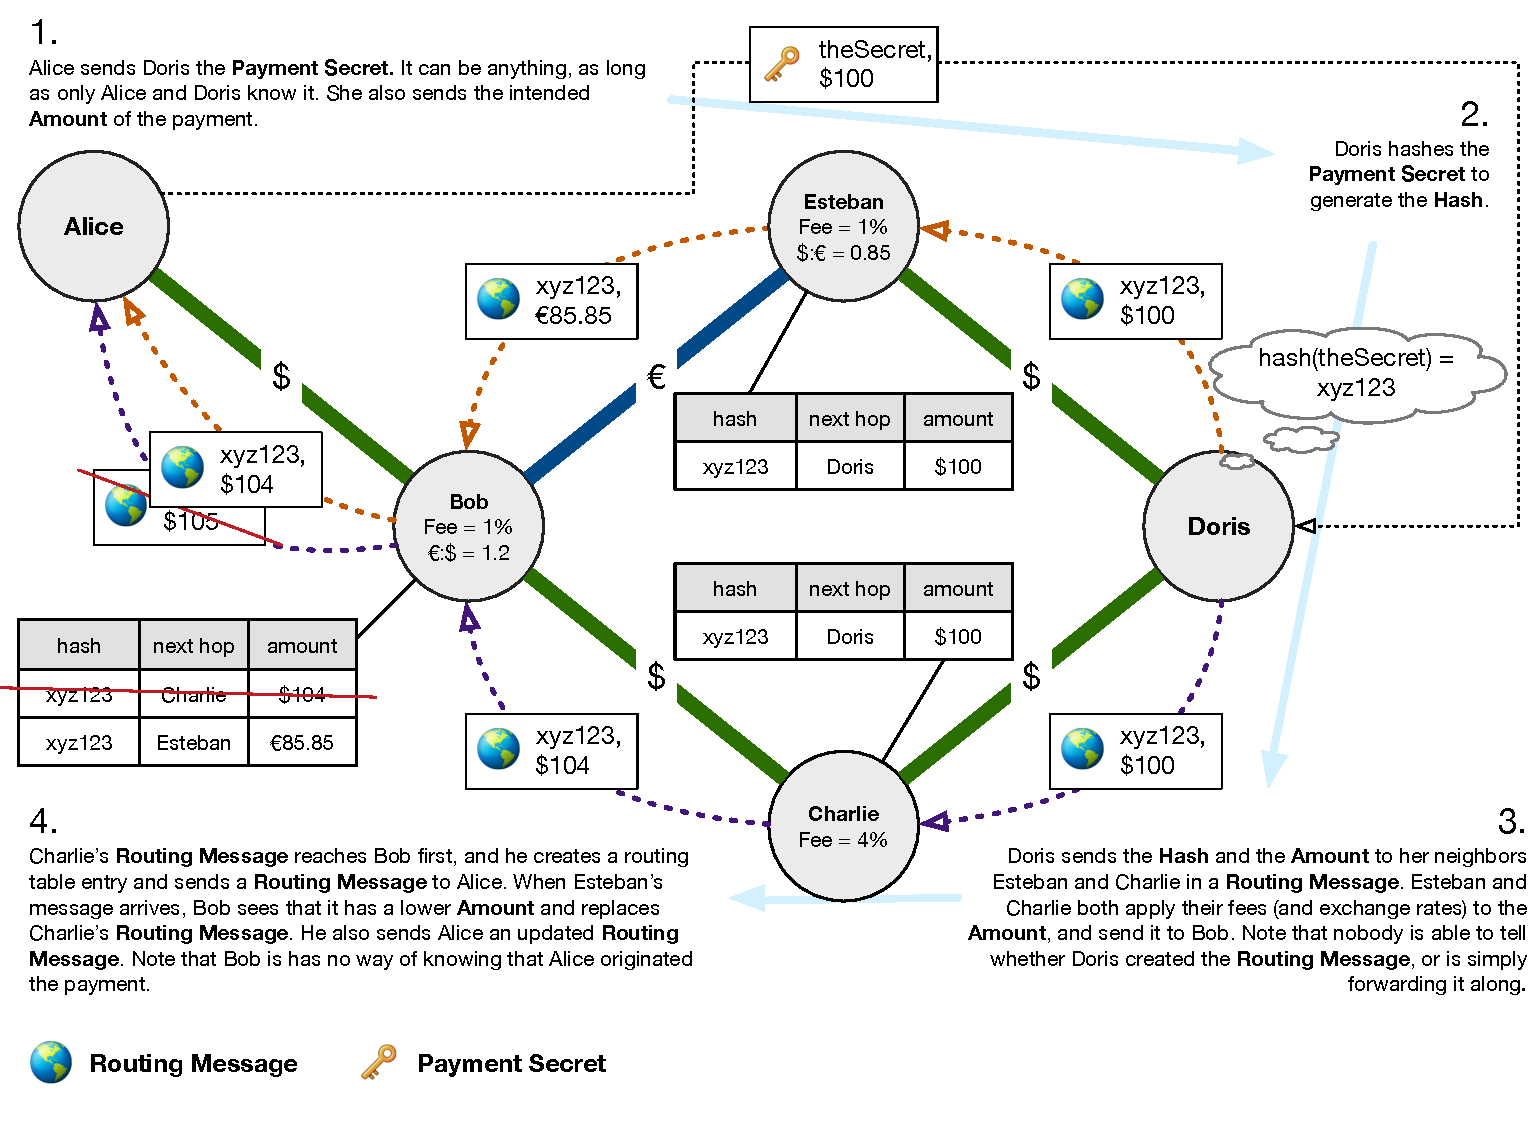
\includegraphics[width=1.5\textwidth]{routing.pdf}}
\caption{Finding a payment route}
\end{figure}

\begin{figure}[H]
\centering
\makebox[\textwidth][c]{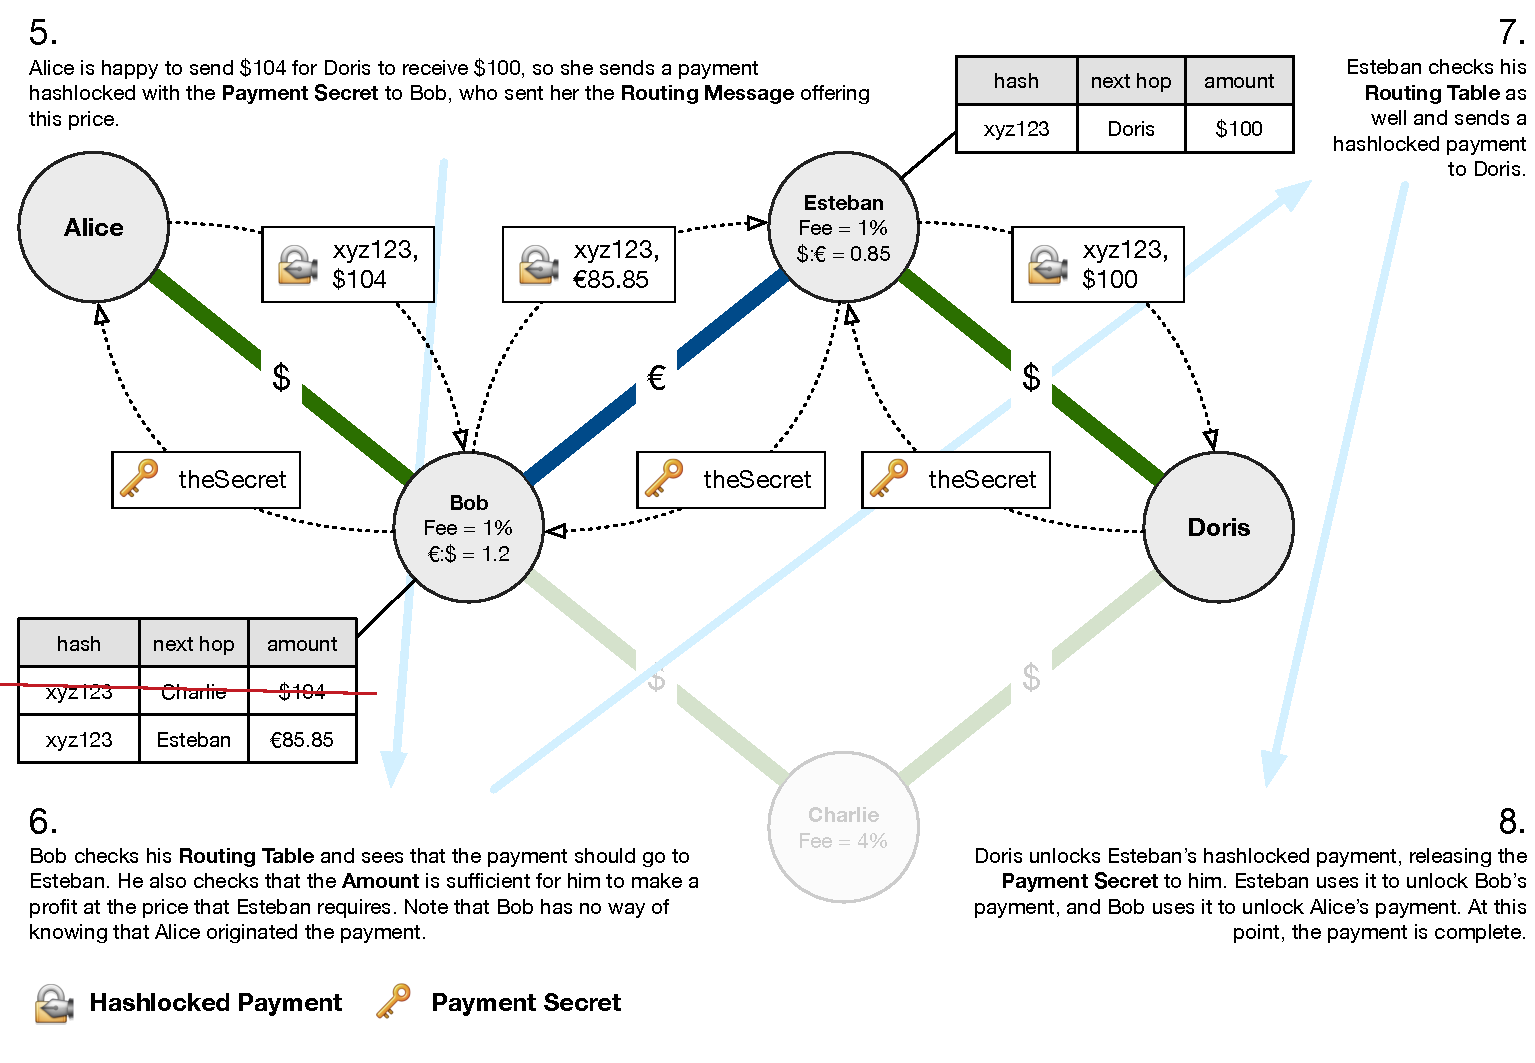
\includegraphics[width=1.5\textwidth]{payment.pdf}}
\caption{Sending a hashlocked payment along a route}
\end{figure}

\pagebreak

\printglossaries

\section*{Acknowledgements}
Zackary Hess, for coming up with much of the definition of the \textbf{Basic Channel} as part of Flying Fox\cite{flyingfox}, a channel-based cryptocurrency and prediction market. Jae Kwon, for years of advice and guidance on the theory, implementation, and philosophy of cryptocurrency. Anke Tremback, for editing the first complete draft of this paper. Alice Townes, for editing and feedback from a legal and finance perspective.


\begin{thebibliography}{99}

\bibitem{interledger}
\emph{A Protocol for Interledger Payments}\\
Stephan Thomas, Evan Schwartz\\
\texttt{https://interledger.org/interledger.pdf}\\
2015

\bibitem{btcwiki}
\emph{Micropayment Channel}\\
Bitcoin Wiki Contributors\\
\texttt{https://bitcoin.org/en/developer-guide\#micropayment-channel}\\
2014

\bibitem{bitcoinj}
\emph{[ANNOUNCE] Micro-payment channels implementation now in bitcoinj}\\
Mike Hearn\\
\texttt{https://bitcointalk.org/index.php?topic=244656.0}\\
2013

\bibitem{blueadept}
\emph{Decentralized networks for instant, off-chain payments}\\
Alex Akselrod\\
\texttt{https://en.bitcoin.it/wiki/User:Aakselrod/Draft}\\
2013

\bibitem{amiko}
\emph{Amiko Pay}\\
C. J. Plooy\\
\texttt{http://cornwarecjp.github.io/amiko-pay/doc/amiko\_draft\_2.pdf}\\
2013

\bibitem{duplexchannels}
\emph{A Fast and Scalable Payment Network with Bitcoin Duplex Micropayment Channels}\\
Christian Decker, Roger Wattenhofer\\
\texttt{http://www.tik.ee.ethz.ch/file/716b955c130e6c703fac336ea17b1670/\\duplex-micropayment-channels.pdf}\\
2015

\bibitem{lightning}
\emph{The Bitcoin Lightning Network: Scalable Off-Chain Instant Payments}\\
Joseph Poon, Thaddeus Dryja\\
\texttt{https://lightning.network/lightning-network-paper.pdf}\\
2015

\bibitem{aodv}
\emph{Ad-hoc On-Demand Distance Vector Routing}\\
Charles E. Perkins, Elizabeth M. Royer\\
\texttt{https://www.cs.cornell.edu/people/egs/615/aodv.pdf}\\

\bibitem{ethereum}
\emph{A Next-Generation Smart Contract and Decentralized Application Platform}\\
Vitalik Buterin\\
\texttt{https://github.com/ethereum/wiki/wiki/White-Paper}\\
2014

\bibitem{tendermint}
\emph{Tendermint: Consensus without Mining}\\
Jae Kwon\\
\texttt{http://tendermint.com/docs/tendermint.pdf}\\
2015

\bibitem{flyingfox}
\emph{Flying Fox}\\
Zackary Hess\\
\texttt{https://github.com/BumblebeeBat/FlyingFox}\\
2015

\end{thebibliography}

\end{document}